% !TEX root = ../sethomas_thesis_main.tex
\documentclass[border=1mm,
               class=article
               preview]{standalone}
\usepackage{tikz}
\usepackage[percent]{overpic}   % For inserting figures within a figure
\usepackage{siunitx}
\usepackage{pict2e}
%%%%%%%%%%%%%%%%%%%%%%%%%%%%%%%%%%%%

% Inserts a scale bar into an image
% Optional argument 1: the colour of the bar and text
% Argument 2: an \includegraphics command
% Argument 3: the real world width of the image
% Argument 4: the length of the scale bar in pixels
% Argument 5: the length of the scale bar in mm
\newcommand{\scalebar}[5][white]{
 \begin{tikzpicture}
  \node[anchor=south west,inner sep=0] (image) { #2 };
  \begin{scope}[x={(image.south east)},y={(image.north west)}]
   \draw [#1, line width=0.4em] (0.04,1.2em) -- node[above,inner sep=0.3em, font=\normalsize] {\SI{#5}{\milli \meter}} (#5*#4/#3+0.04,1.2em);
  \end{scope}
 \end{tikzpicture}
}

\begin{document}
\begin{tikzpicture}
    \pgfmathsetmacro{\yTopPicture}{4.9}
    \pgfmathsetmacro{\xFigLetter}{0.05}
    \pgfmathsetmacro{\yFigLetter}{0.93}
    \pgfmathsetmacro{\e}{0.5mm}

    \node[anchor=south west,inner sep=0] (graph) at (0,\yTopPicture) {\scalebar{
    \begin{overpic}[trim={0 10cm 0 25cm},clip,width=0.98\columnwidth]{images/chap7/proto_open.jpeg}
        \put(0,0){\color{myred}\linethickness{0.5mm}% Middle box
        \polygon(31,30)(31,36)(66,36)(66,30)}
        \put(0,0){\color{myred}\linethickness{0.5mm}% Zoom lines
        \polygon(31,30)(37,15.9)(97.7,15.9)(66,30)}
        \put(37,1){\color{myred}\linethickness{0.5mm}% Zoomed image
        \frame{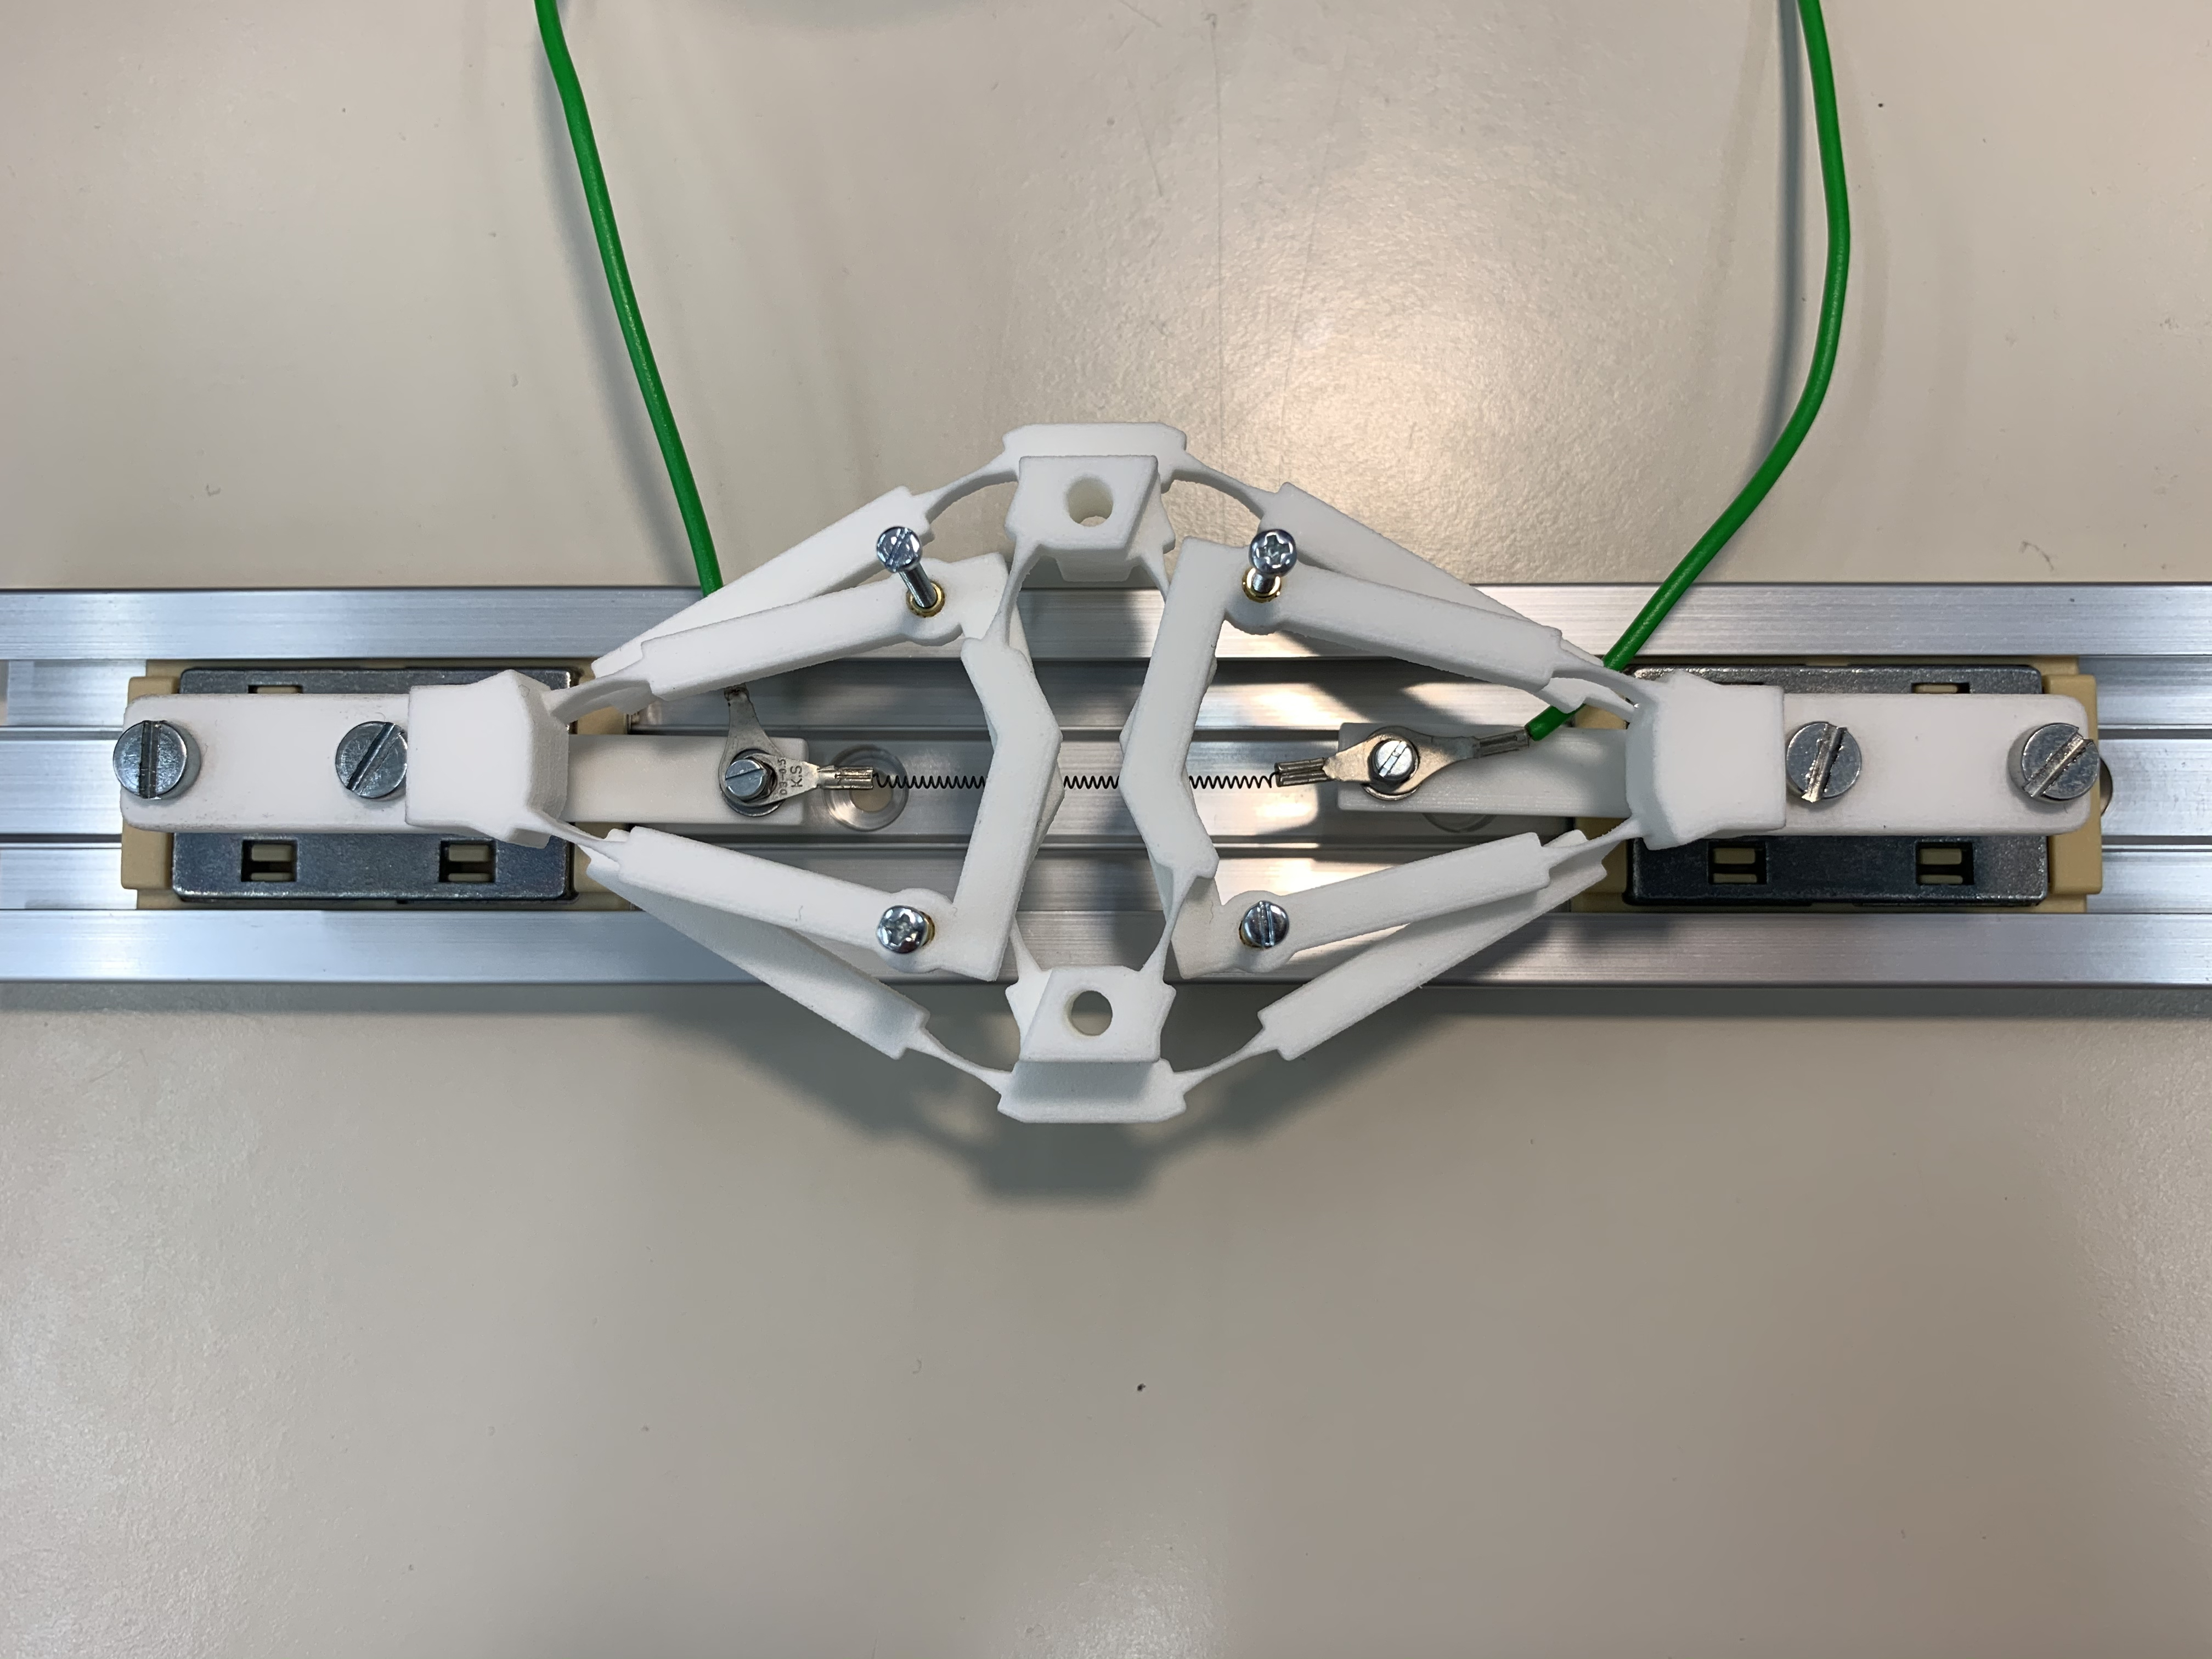
\includegraphics[trim={45cm 50cm 48cm 45cm},clip,width=0.6\columnwidth]{images/chap7/proto_open.jpeg}}}
    \end{overpic}
    }{197.8}{1}{20}};
    \begin{scope}[x={(graph.south east)},y={(graph.north west)}]
       \node[align=left] at (\xFigLetter,\yFigLetter) {\Large \color{white}(a)};
    \end{scope}

     \node[anchor=south west,inner sep=0] (graph1) at (0.06,-3.4){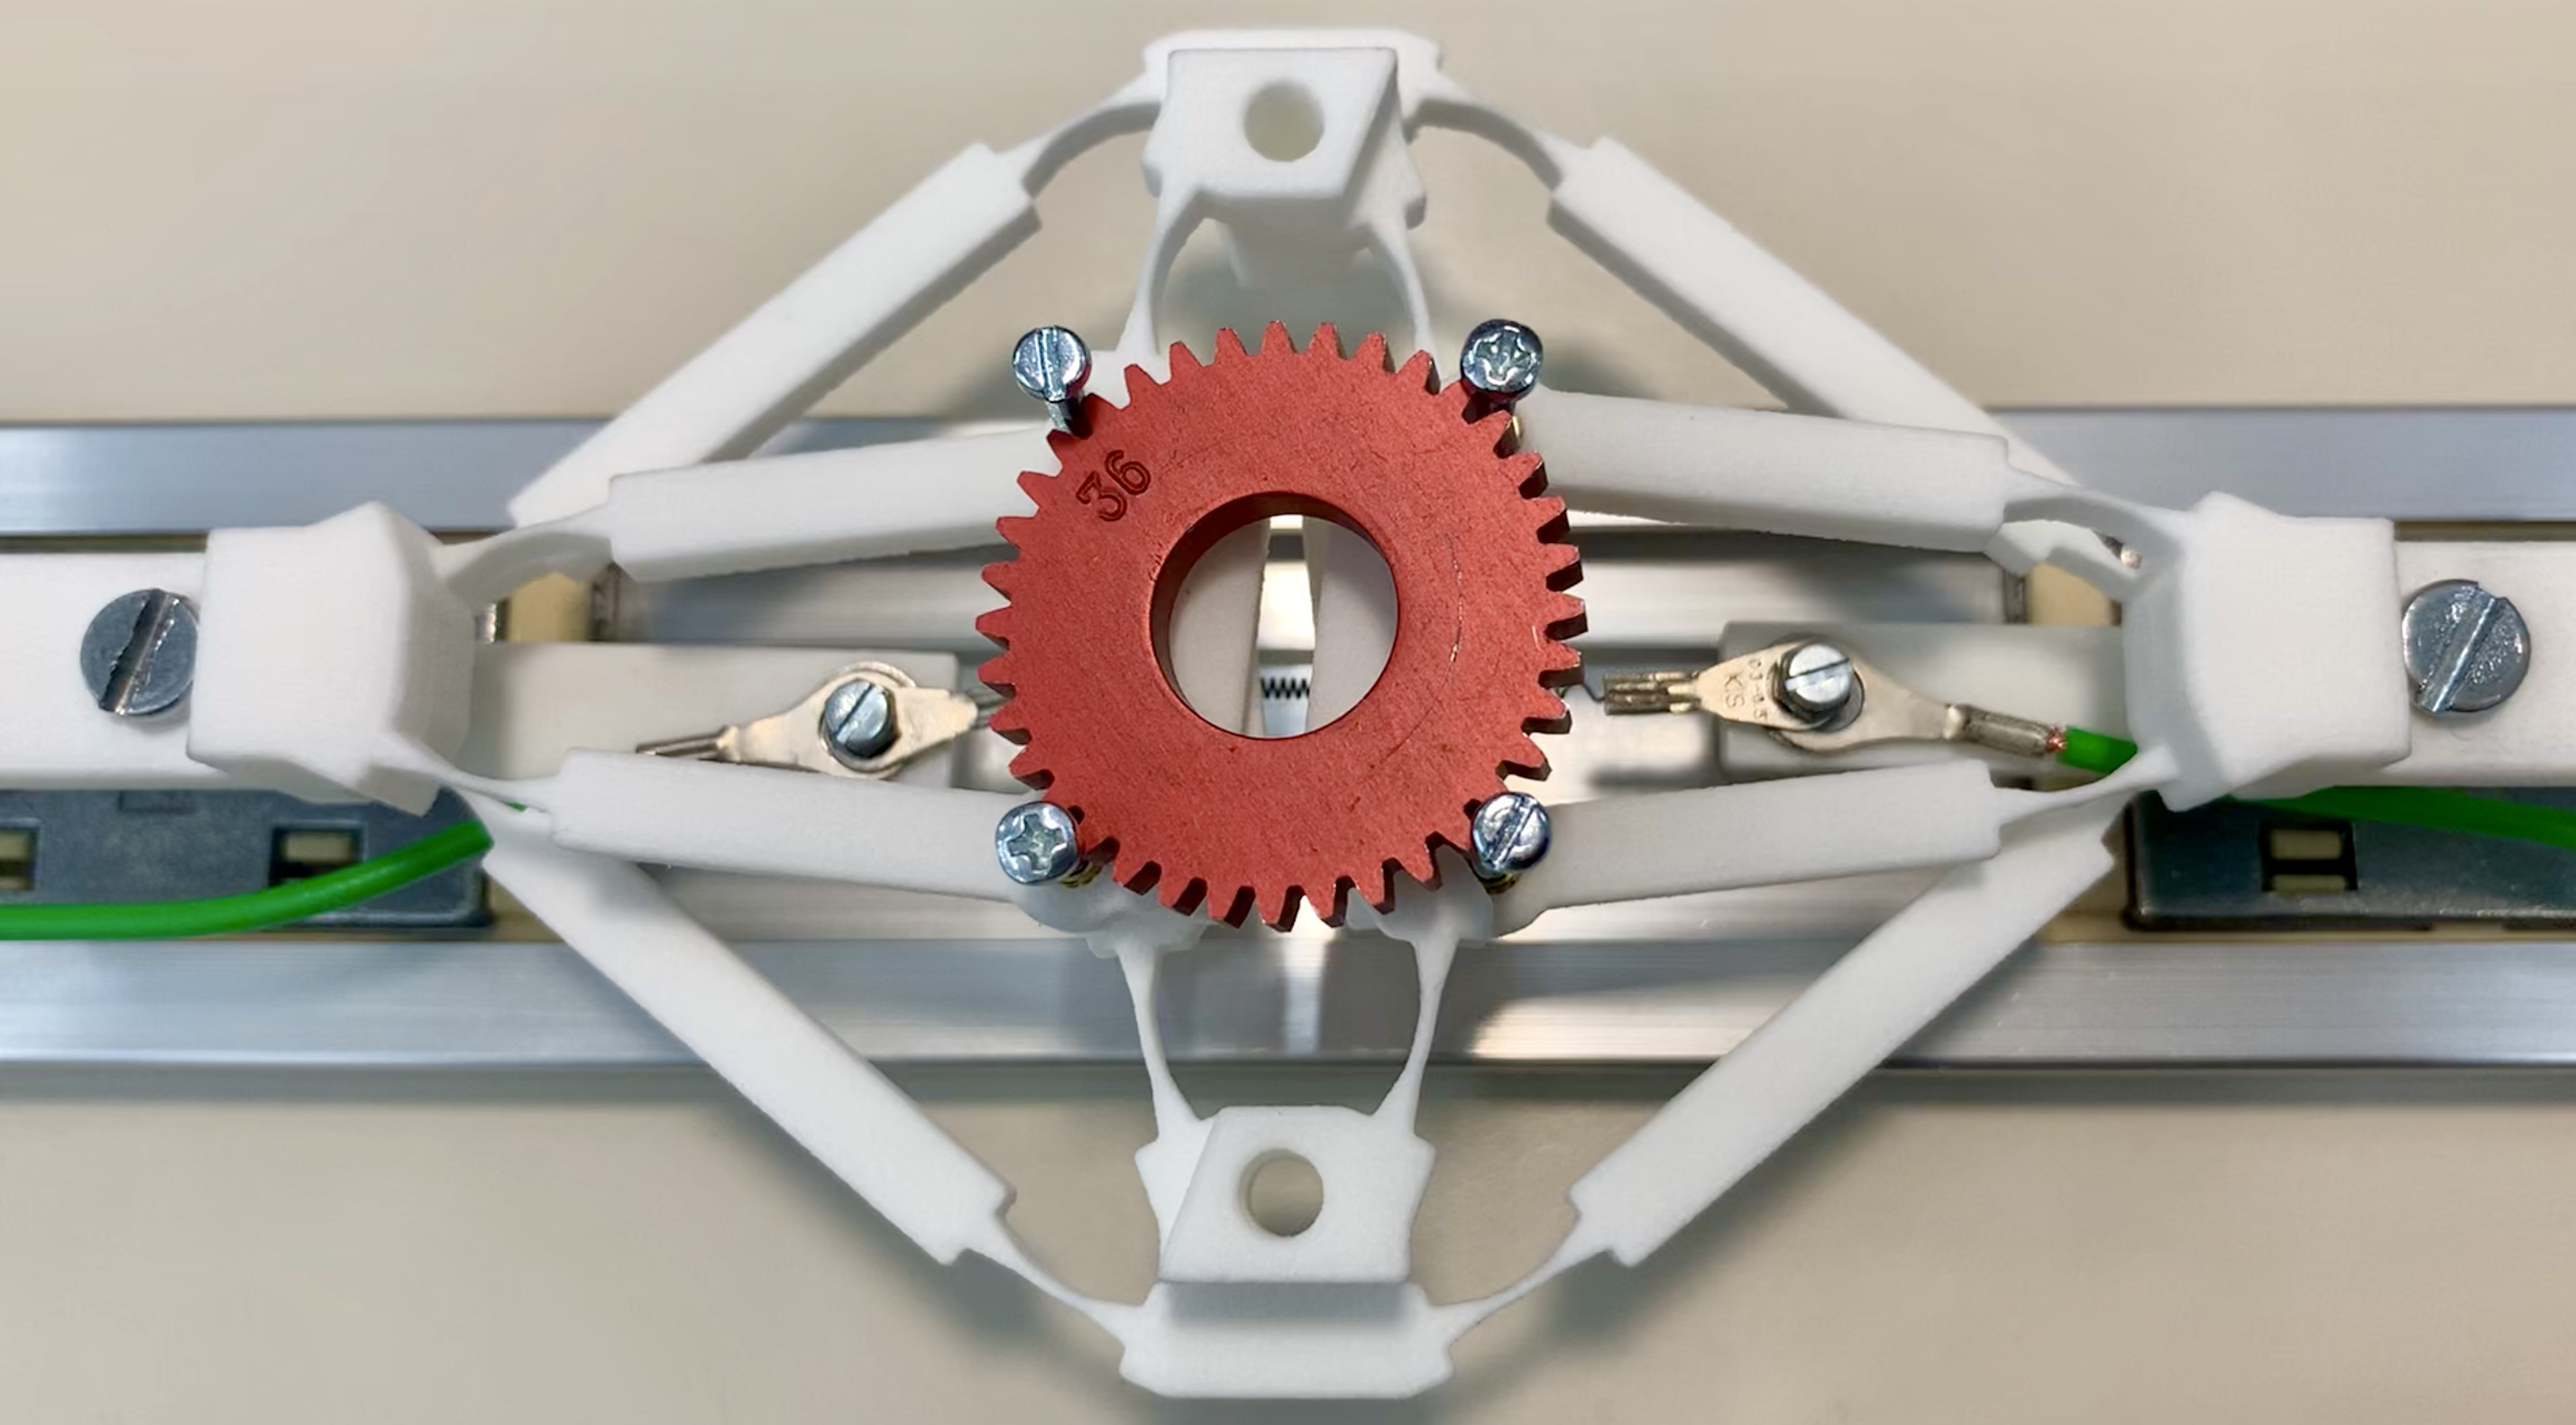
\includegraphics[width=0.98\columnwidth]{images/chap7/closed_with_object.jpeg}};
     \begin{scope}[x={(graph1.south east)},y={(graph1.north west)}]
        \node[align=left] at (\xFigLetter,\yFigLetter) {\Large \color{white}(b)};
     \end{scope}


% \draw[thick,cyan,arrows={-Triangle[angle=90:10pt,cyan,fill=cyan]}] (1.7,\yTopPicture+2.8) -- (3.1,\yTopPicture+2.8);
% \draw[help lines] (0,0) grid (8,4); % $$$$$$$$$$$$$ HELPS A LOT FOR COORDINATES $$$$$$$
 \end{tikzpicture}
\end{document}
